%%%%%%%%%%%%%%%%%%%%%%%%%%%%%%%%%%%%%%%%%%%%%%%%%%%%%%%%%%%%%%%%%%%%%%%%%%%%%%%
% BAND ASSIGN
%%%%%%%%%%%%%%%%%%%%%%%%%%%%%%%%%%%%%%%%%%%%%%%%%%%%%%%%%%%%%%%%%%%%%%%%%%%%%%%
\begin{figure}
\centering
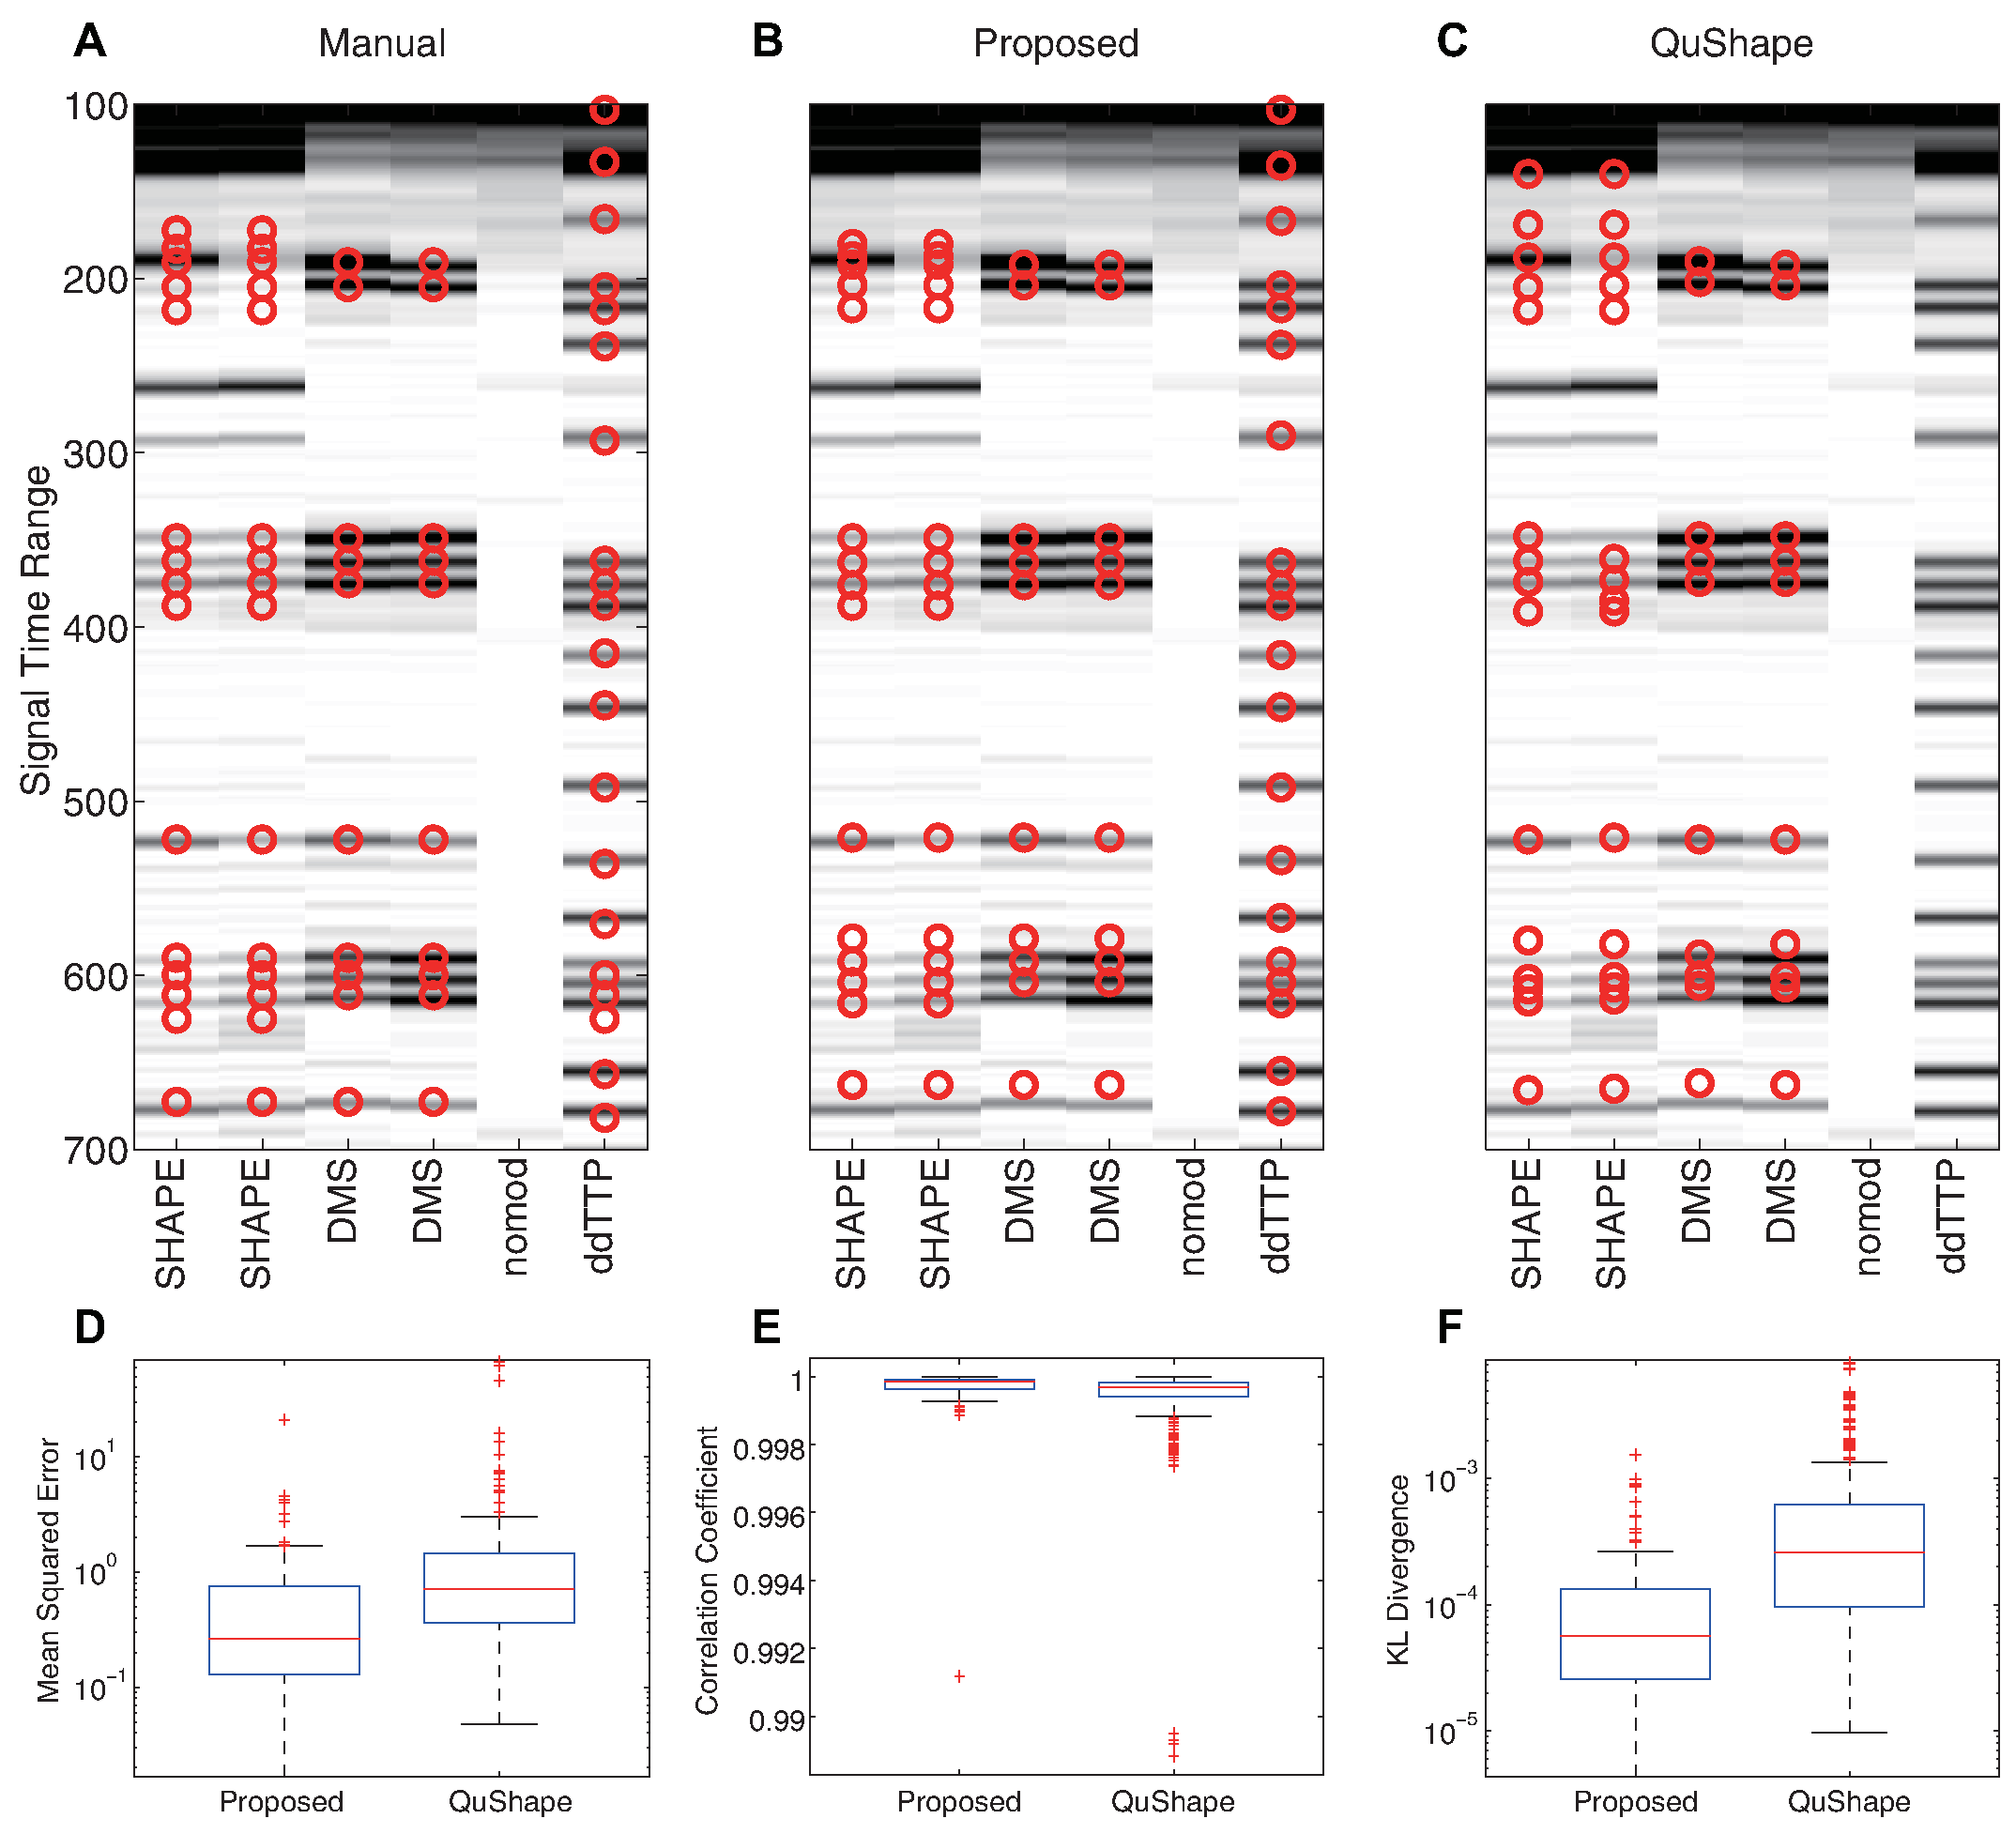
\includegraphics[width=0.9\linewidth]{../figures/result_band_assign4}
\caption{Determination of band locations. (A) Reference (manual) annotation. Red circles represent band locations. (B) The band locations determined by the proposed method. (C) The band locations found by QuShape~\citep{Karabiber2013}. (D) Mean squared error (MSE) (E) Pearson's correlation coefficient (F) KL divergence}
\label{f:band-assign}
\end{figure}
%%%%%%%%%%%%%%%%%%%%%%%%%%%%%%%%%%%%%%%%%%%%%%%%%%%%%%%%%%%%%%%%%%%%%%%%%%%%%%%

%%%%%%%%%%%%%%%%%%%%%%%%%%%%%%%%%%%%%%%%%%%%%%%%%%%%%%%%%%%%%%%%%%%%%%%%%%%%%%%
% PEAK AREA
%%%%%%%%%%%%%%%%%%%%%%%%%%%%%%%%%%%%%%%%%%%%%%%%%%%%%%%%%%%%%%%%%%%%%%%%%%%%%%%
\begin{figure}
\centering
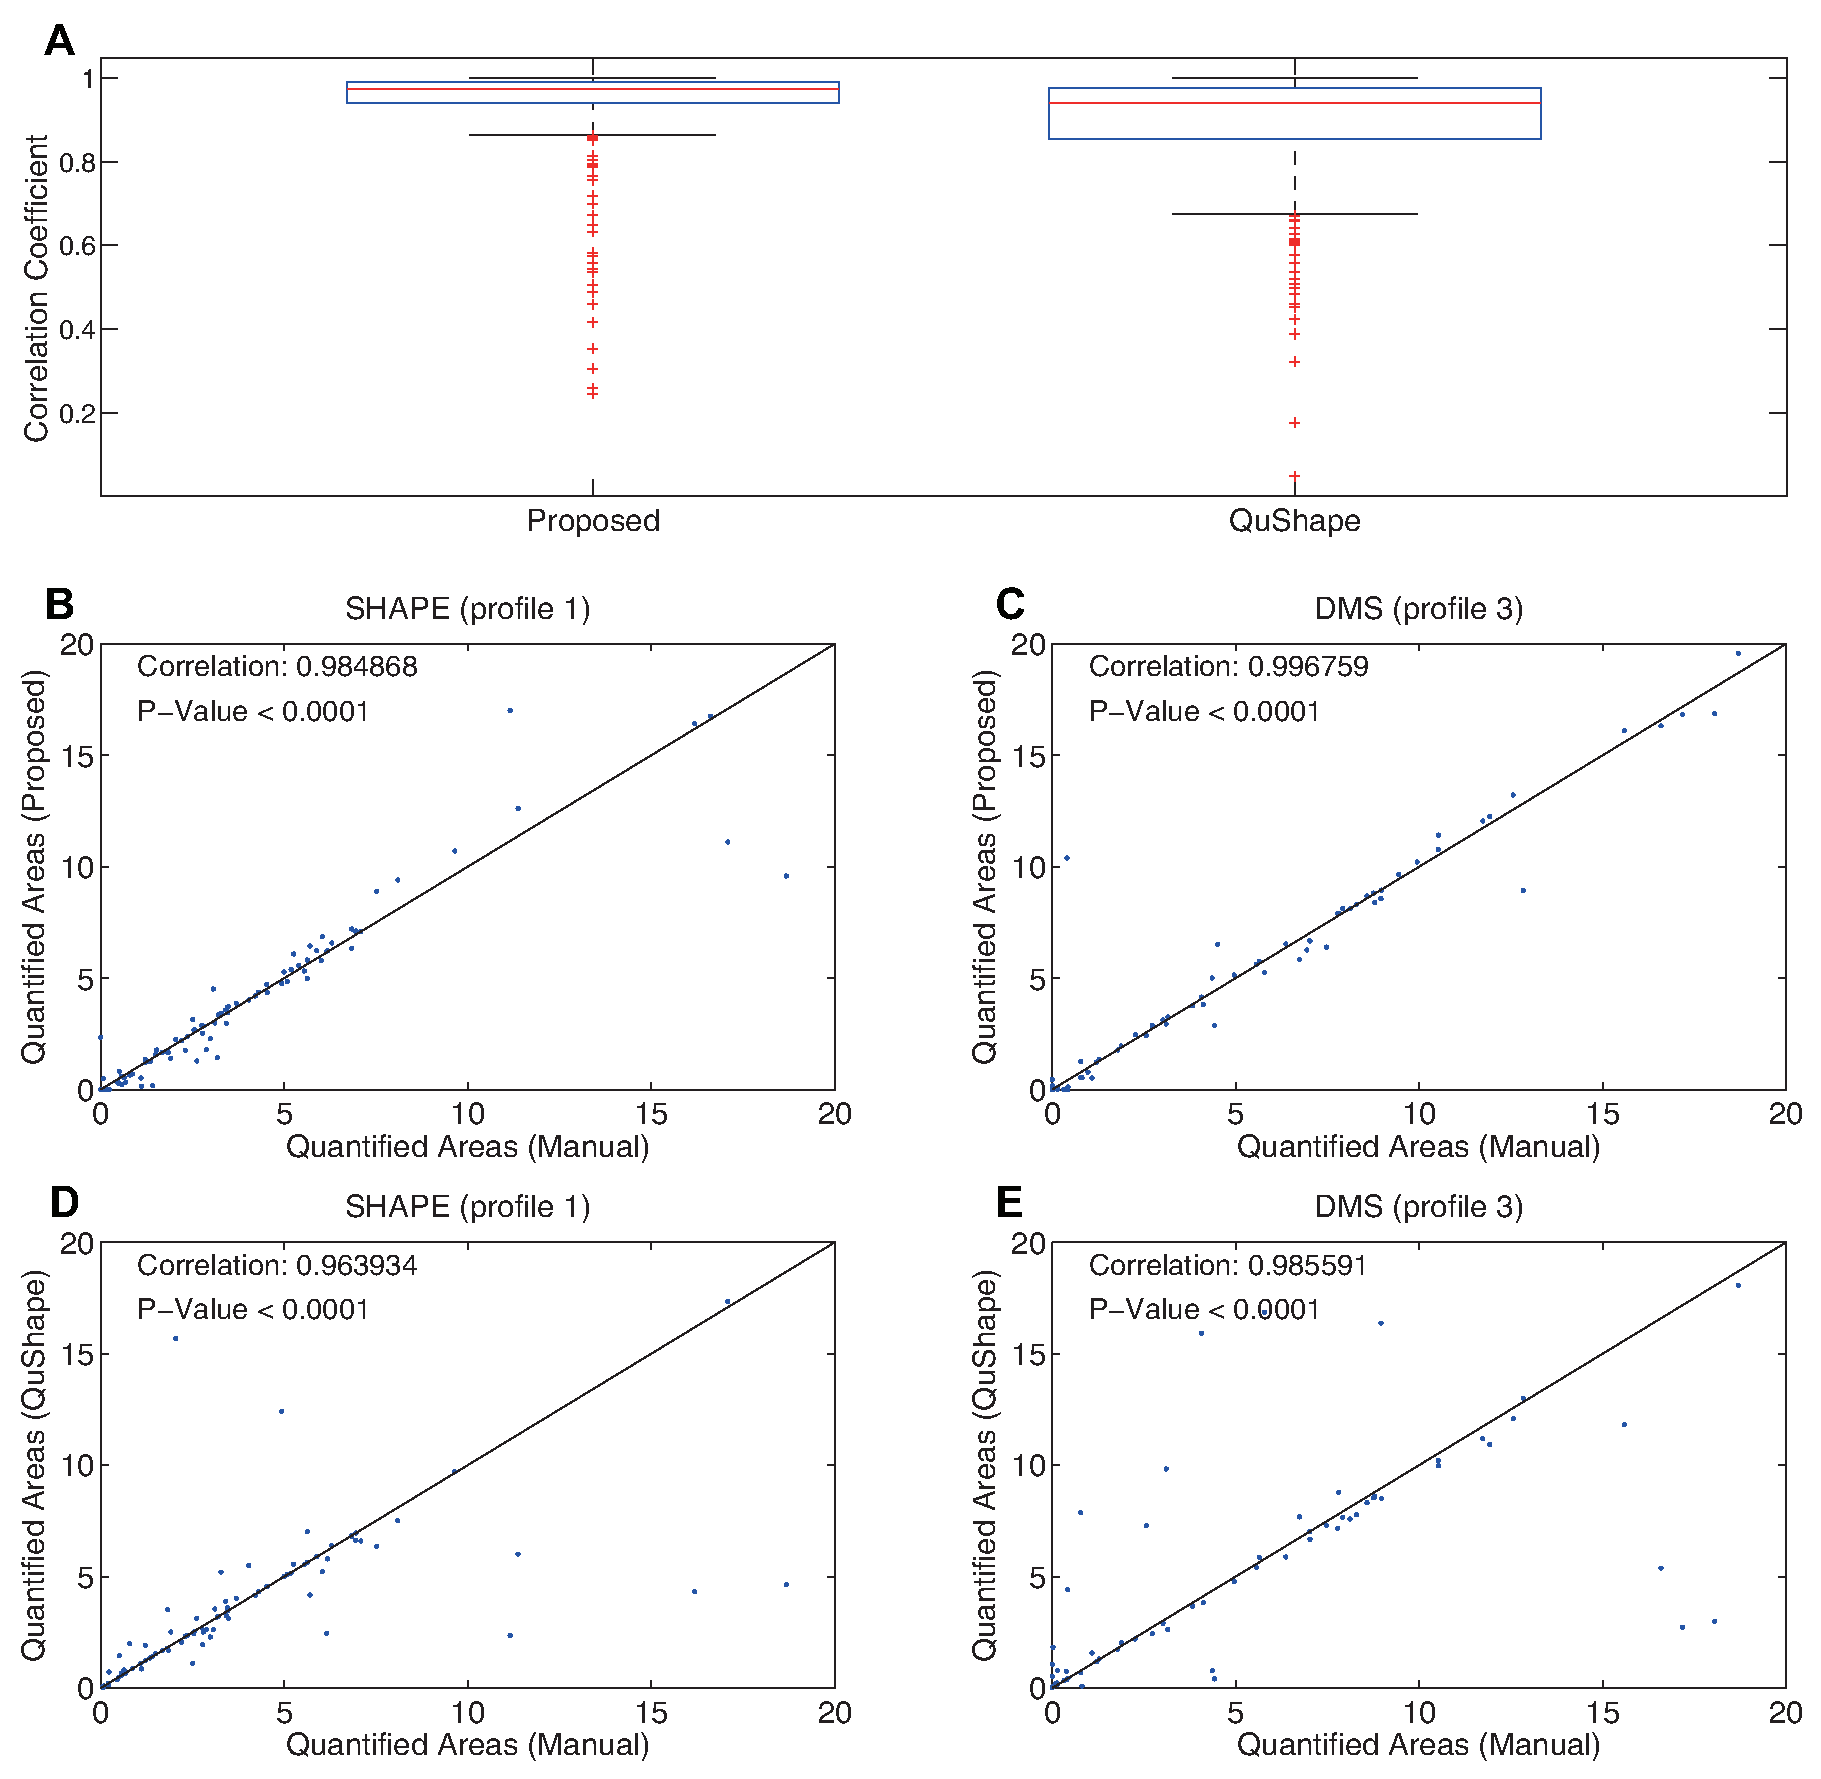
\includegraphics[width=0.9\linewidth]{../figures/result_peak_area4}
\caption{Accuracy of quantifying peak areas. (\textbf{a}) The left box plot represents the distribution of the Pearson's correlation coefficients between the manually quantified areas and those quantified by the proposed method over the 95 data sets. The right box plot shows the distribution of the correlation coefficients between the areas quantified manually and by QuShape. (\textbf{b}--\textbf{c}) Correlation of the reference and the quantified areas by the proposed method for data set `FMN Binding Branches' is shown for profiles 1 (SHAPE) and 3 (DMS). (\textbf{d}--\textbf{e}) Correlation of the reference and the areas quantified by QuShape for the same data set.
}
\label{f:peak-area}
\end{figure}
%%%%%%%%%%%%%%%%%%%%%%%%%%%%%%%%%%%%%%%%%%%%%%%%%%%%%%%%%%%%%%%%%%%%%%%%%%%%%%%

\newcommand{\bP}{{\mathbf{P}}}


\subsection{Robust determination of band positions}\label{ss:band-position}
Figure~\ref{f:band-assign}(a)--(c) shows the electrophoretic profiles annotated with band locations by three different methods: reference, proposed, and QuShape~\citep{Karabiber2013}, respectively. The reference annotation was based an expert assignments carried out at the time of data acquisition~\citep{lee2014eterna} QuShape was chosen as the comparison target for its superior accuracy in band annotation relative to other software we tested, FAST and ShapeFinder (data not shown); nomod and ddTTP profiles were used as references (RXS1, BGS1) while running QuShape. Visual inspection suggests that the proposed method produces annotations more compatible with the reference. In this profile, the annotation determined by QuShape deviates from the reference position, particularly near the beginning of sequence.

To generally and quantitatively assess the accuracy of automated band annotation, we applied the proposed method and QuShape to 95 data sets acquired in the EteRNA project (Table \ref{t:data}). For both methods, we computed the mean squared error (MSE) of the band locations determined by the proposed method with respect to the reference locations, in units of average distance between locations. For a sense of scale, the typical MSE achieved by expert annotation is 0.15, based on comparisons of different expert's annotations and of CE-based data to Illumina-based measurements where sequence annotation is unambiguous \citep{Kladwang2014}; see Supplemental Fig. S1. Furthermore, in our experience, a band annotation result with MSE lower than 0.5 typically requires no or a small number single-click corrections. The box plots in Figure~\ref{f:band-assign}(d)--(f) and individual MSE values (Supplemental Tables S1 and S2) reveal that the proposed method outperforms QuShape across the data sets. For example, the median MSE of the proposed method is 0.37 compared to 1.8 from QuSHAPE. As separate metrics of accuracy, we measured the Pearson's correlation coefficient and the Kullback-Leibler (KL) divergence between the reference and computationally determined band positions.  Again, the average correlation coefficient of the proposed method is 1.92 times closer to 1, and the average KL divergence is 5.49 times smaller. These results quantitatively confirm what we observed qualitatively on using these tools: significantly less manual intervention is needed with the proposed method compared to QuShape.


\subsection{Accurate peak-area quantification}\label{ss:peak-area}
In the RNA structure mapping pipeline, the band annotation is followed by peak deconvolution, which fits each band with a Gaussian curve and produces the quantified area of the band. To see how these final band quantification results are impacted by the band annotation method, we calculated Pearson's correlation coefficients between band areas quantified based on the band annotation found by the proposed method and those quantified based on the reference annotation. We also repeated the calculation with the band intensities quantified by QuShape. For fair comparison, we applied the same peak deconvolution software (HiTRACE; \citealp{Yoon2011}) to these three methods.

As one example, Figure~\ref{f:peak-area}(b) and (c) shows the correlation of results between the proposed method and reference for a specific data set (FMN Binding Branches) for two chemical modification strategies (SHAPE and DMS).and Figure~\ref{f:peak-area}(d) and (e) shows the correlation between the QuShape and reference results, which are visually worse in both cases. Over all the data sets, Figure~\ref{f:peak-area}(a) and Supplemental Table S1 gives the distribution of the Pearson's correlation coefficients. The median correlation coefficient for the proposed method is 0.969 which is higher than that for QuShape, 0.896, and the distribution for the proposed method shows smaller variance. This observation suggests that using the proposed band annotation can significantly enhance the accuracy of band quantification. 


\begin{comment}
%%%%%%%%%%%%%%%%%%%%%%%%%%%%%%%%%%%%%%%%%%%%%%%%%%%%%%%%%%%%%%%%%%%%%%%%%%%%%%%
% HDV RESULT
%%%%%%%%%%%%%%%%%%%%%%%%%%%%%%%%%%%%%%%%%%%%%%%%%%%%%%%%%%%%%%%%%%%%%%%%%%%%%%%
\begin{figure}
\centering
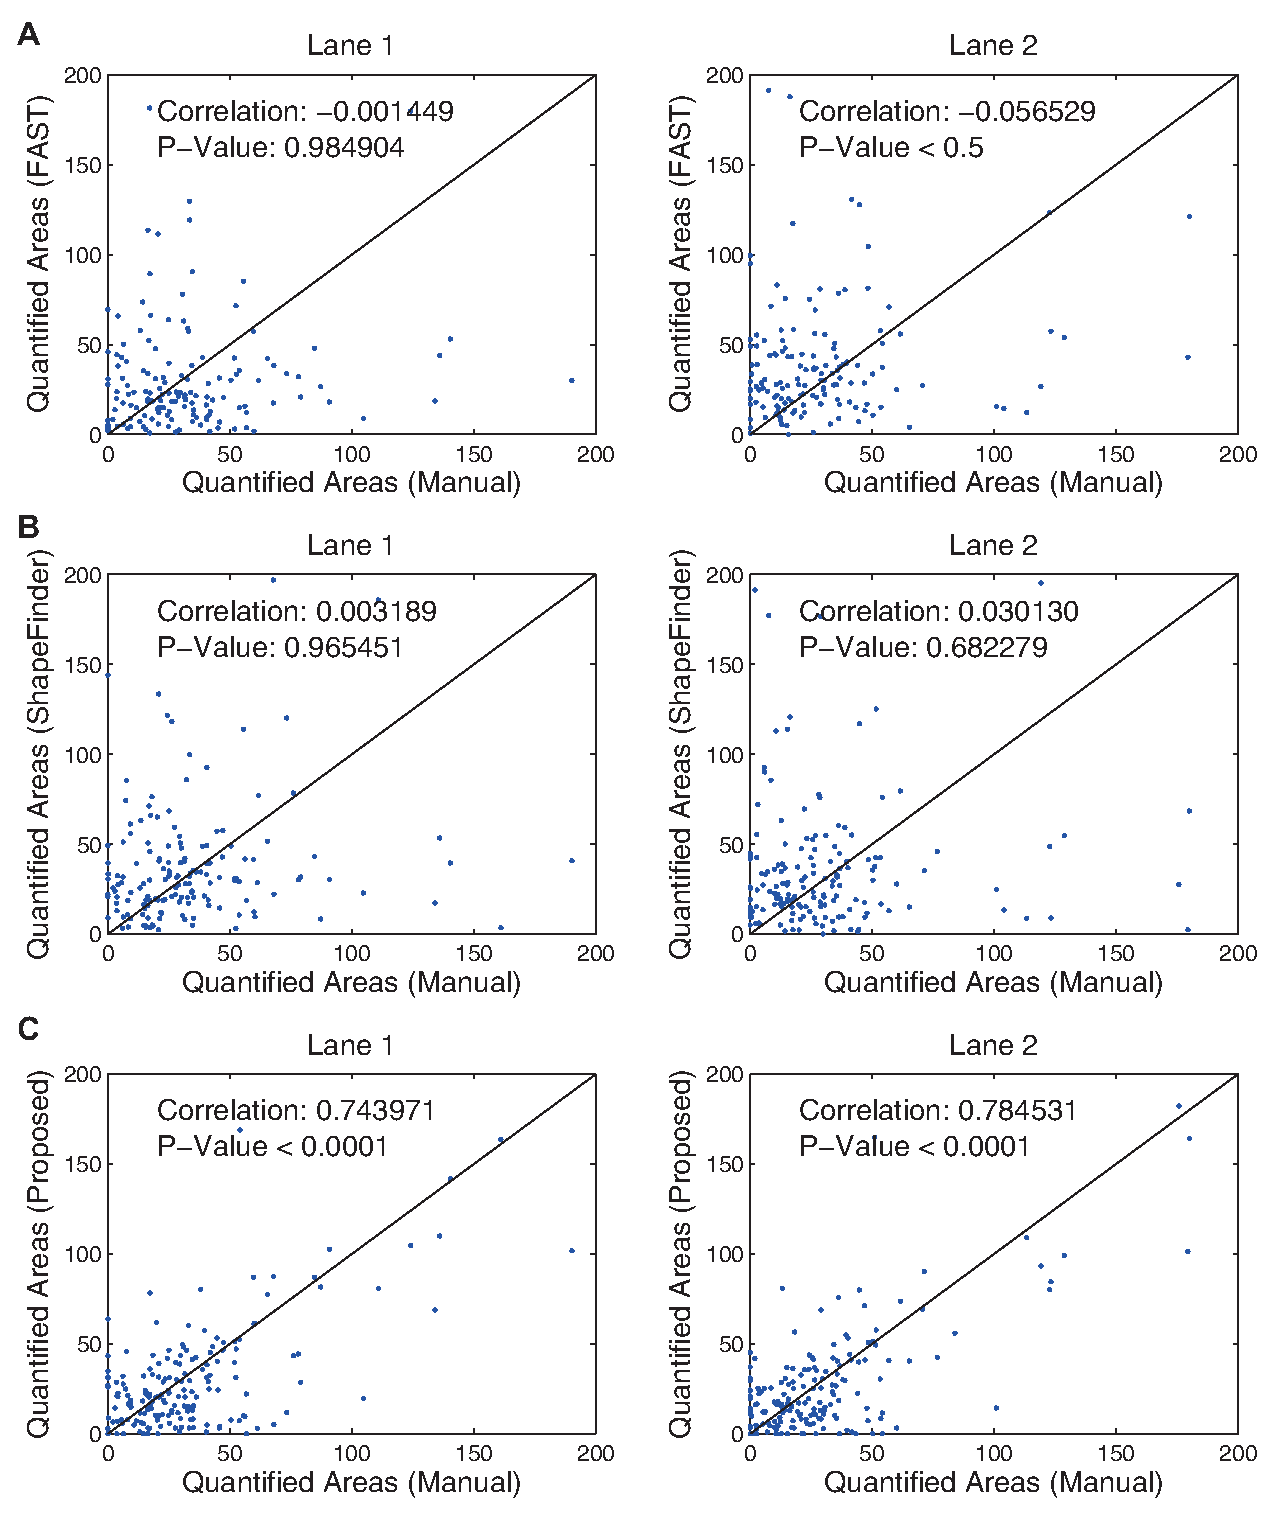
\includegraphics[width=\linewidth]{../figures/result_hdv_result3}
\caption{Assessing band annotation results from 187-nt HDV data set. (\textbf{a}--\textbf{c}) Correlation between the areas quantified manually and by FAST, ShapeFinder, and the proposed method over two profiles, respectively.}
\label{f:hdv-result}
\end{figure}
%%%%%%%%%%%%%%%%%%%%%%%%%%%%%%%%%%%%%%%%%%%%%%%%%%%%%%%%%%%%%%%%%%%%%%%%%%%%%%%

\subsection{Results in longer RNAs}
To test the proposed method with a longer RNA molecule, we used a chemical mapping data set from a study on the NMIA (SHAPE) modification of the hepatitis delta virus (HDV) ribozyme (187-bp). For this data set, we included the FAST software~\citep{Pang2011} in comparison. FAST has a hard-wired requirement for ddGTP as reference ladder and could not be used for the other 95 data sets presented earlier (they contained ddTTP profiles instead).

We repeated the experiments presented in Sections~\ref{ss:band-position} and \ref{ss:peak-area} for this HDV data set. The proposed method substantially outperformed FAST and ShapeFinder in terms of MSE (proposed: 1.14, ShapeFinder: 321.03, and FAST: 142.12), although its MSE is higher than those for shorter sequences (Figure~\ref{f:band-assign}(d)). 


\emph{I DON'T THINK WE SHOULD SHOW THESE R VALUES -- EVEN FOR OUR NEW METHOD, THEY ARE NOT ACCEPTABLE}
Figure~\ref{f:hdv-result}(a)-(c) shows the correlation of the reference areas with band areas quantified by the proposed method, ShapeFinder, and FAST, respectively. The band areas quantified by the proposed method show a high degree of correlation with the reference ($r= 0.744$ and $0.785$), whereas the two other methods give unsatisfactory results ($r< 0.05$). 

Figure~\ref{f:hdv-result-detail} shows the distribution of errors in predicted band locations over the position of residues in the HDV data set. This is to check if there is any systematic bias in band annotation on the residue position. The middle diagram represents the mapping between the reference band locations and those determined by the proposed method. The upper and lower plots show the position errors for the proposed method and FAST, respectively. For the proposed method, the errors near the start location tends to be larger than those in the middle. According to our experience, there exist very high-intensity bands in the starting and ending portion of a profile, which hinders even the manual band annotation. The larger error near these segments in a profile may be due to these high-intensity bands. The error pattern in the result from FAST shows a different pattern, and the largest errors appear near residues 40--50. Overall, the errors from the proposed method were consistently lower than those from FAST.


%%%%%%%%%%%%%%%%%%%%%%%%%%%%%%%%%%%%%%%%%%%%%%%%%%%%%%%%%%%%%%%%%%%%%%%%%%%%%%%
% HDV RESULT DETAIL
%%%%%%%%%%%%%%%%%%%%%%%%%%%%%%%%%%%%%%%%%%%%%%%%%%%%%%%%%%%%%%%%%%%%%%%%%%%%%%%
\begin{figure}
\centering
	\psfrag{r}[][][0.5]{$\rho$}
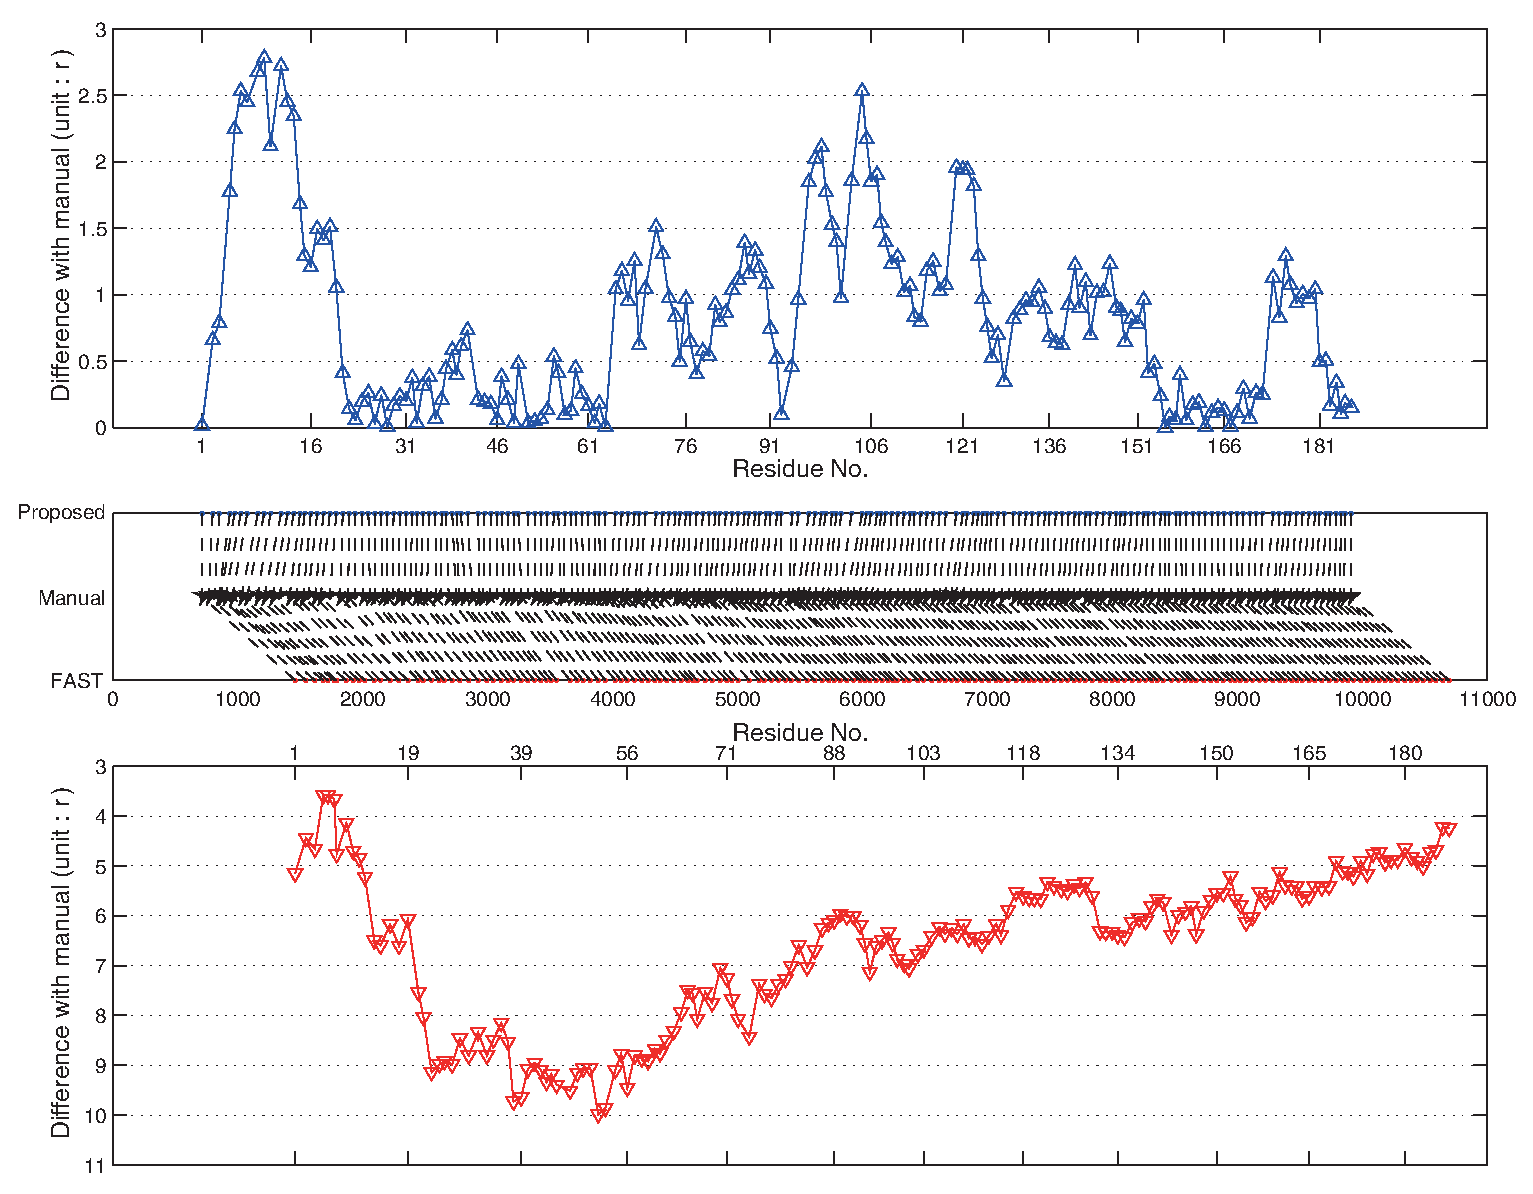
\includegraphics[width=\linewidth]{../figures/result_hdv_result_detail2}
\caption{Error in band positions with respect to the reference band locations for 187-nt HDV data. Upper plot: error over residue positions for the proposed method; middle: mapping between the reference and computationally predicted band locations; lower: error over residue positions for FAST.}
\label{f:hdv-result-detail}
\end{figure}
%%%%%%%%%%%%%%%%%%%%%%%%%%%%%%%%%%%%%%%%%%%%%%%%%%%%%%%%%%%%%%%%%%%%%%%%%%%%%%%
\end{comment}


%%%%%%%%%%%%%%%%%%%%%%%%%%%%%%%%%%%%%%%%%%%%%%%%%%%%%%%%%%%%%%%%%%%%%%%%%%%%%%%
% E-SCORE MSE
%%%%%%%%%%%%%%%%%%%%%%%%%%%%%%%%%%%%%%%%%%%%%%%%%%%%%%%%%%%%%%%%%%%%%%%%%%%%%%%
\begin{figure}
\centering
	\psfrag{x}[][][0.7]{$\escore$-score}
	\psfrag{y}[][][0.7]{$\escore=1$}
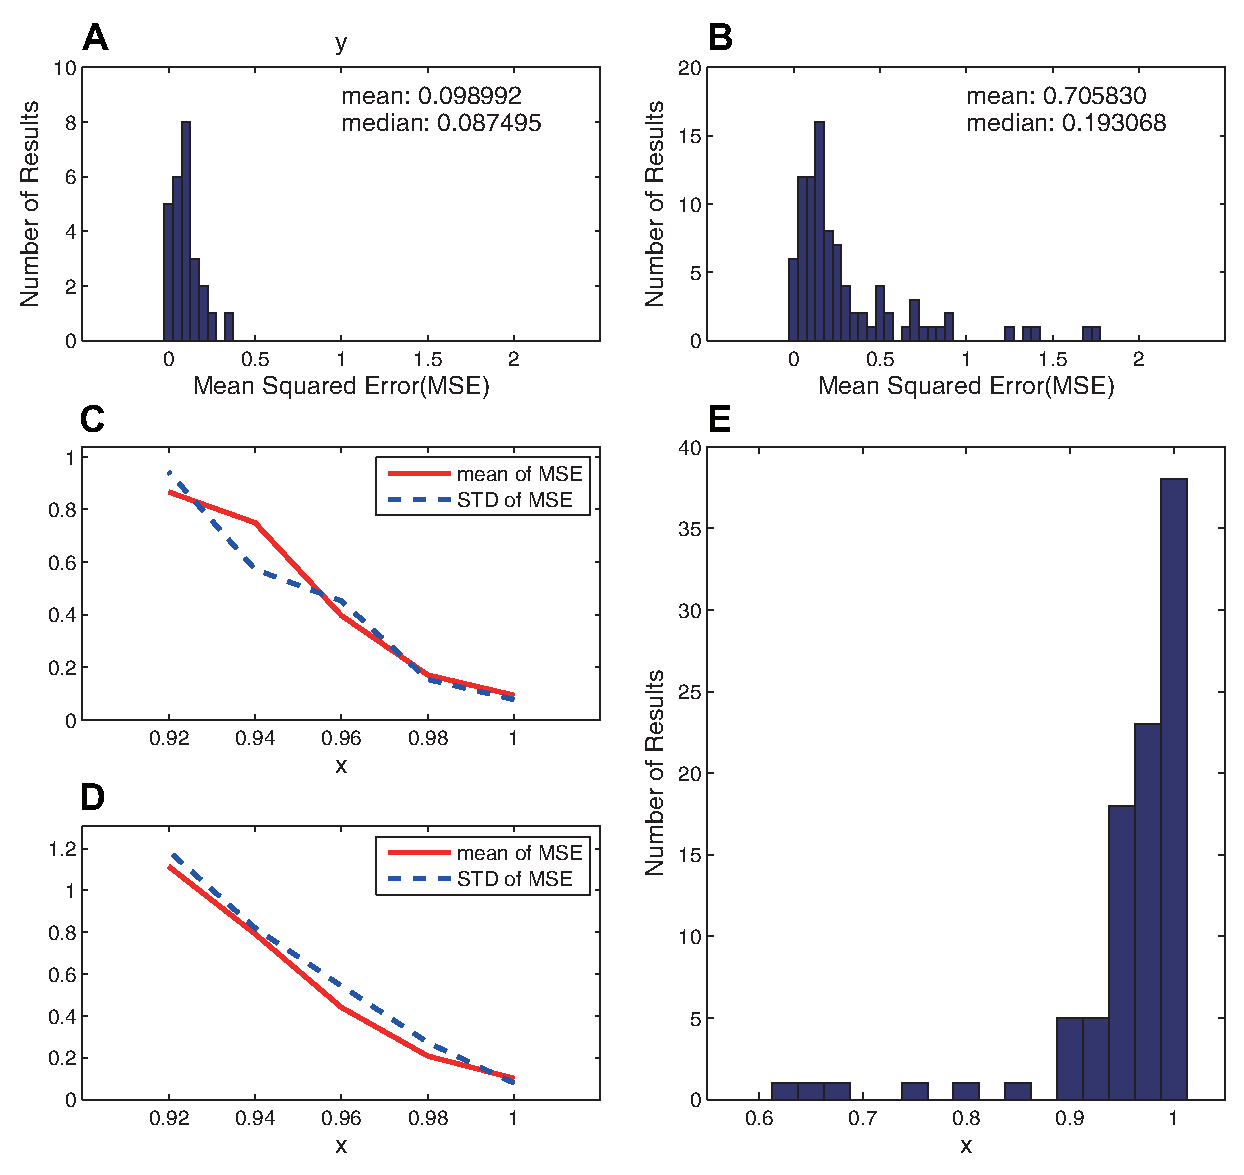
\includegraphics[width=0.9\linewidth]{../figures/result_escore_mse4}
\caption{(\textbf{a}) Distribution of MSE for the results with 1 $\escore$-score. (\textbf{b}) Distribution of MSE for the whole 95 results. (5 results with MSE $> 2$ are ommited for better demonstration) (\textbf{c}) Trends of mean and standard deviation of MSE with respect to $\escore$-score over artificial data generated from a single original data set. (\textbf{d}) Trends of mean and standard deviation of MSE with respect to $\escore$-score for artificial data generated from the whole 95 data sets. (\textbf{e}) Distribution of $\escore$-score over 95 data sets.}
\label{f:escore-mse}
\end{figure}
%%%%%%%%%%%%%%%%%%%%%%%%%%%%%%%%%%%%%%%%%%%%%%%%%%%%%%%%%%%%%%%%%%%%%%%%%%%%%%%

\subsection{Strong correlation between $\escore$-score and MSE}

In Section~\ref{ss:reliability-evaluation}, we proposed $\escore$-score to evaluate the quality of results from our method. We assessed the use of $\escore$-score based on its ability to predict the accuracy of the band annotations compared to gold standard annotations, quantitatively evaluated as mean squared error (MSE). Figure~\ref{f:escore-mse}(a)--(b) show the distribution of the MSEs where (a) only contains results satisfying $\escore = 1$ whereas (b) covers all 95 data sets; consequently the histogram (a) is a subset of histogram (b). It is obvious from the shape of figures that results in (a) are mostly from the left side of (b) implying that the results with high MSE can be filtered out by limiting $\escore$-score. For example, all of 26 results under constraint $\escore=1$ have MSE below 0.5 as shown in (a), reflecting that the constraint $\escore=1$ almost guarantees high quality of band annotations; furthermore, 50 out of 51 results under $\escore>0.97$ have MSE below 0.5 (even the one exception has MSE less than 1.) Since 95 data sets may not be sufficient to conclude on a statistically strong correlation, however, artificial data sets were generated based on the original data sets through random convolution in terms of amplitude and interval for further verification. Figure~\ref{f:escore-mse}(c)--(d) show the trends of mean and standard deviation of MSE with respect to $\escore$-score, where (c) comes from artificial data generated from a single data set whereas artificial data involved in (d) is generated from the whole 95 data sets. The trends shown in (c) and (d) are consistent with the inference from the comparison of (a) with (b) in the sense that a lower $\escore$-score is followed by higher and more capricious distribution of mean squared error. In particular, the trends in (c) support the correlation of $\escore$-score and MSE in a different way from the earlier reasoning by (a)--(b) comparison because only a single data set out of the 95 originals is concerned in (c) unlike in (a) and (b). Figure~\ref{f:escore-mse}(e) shows the histogram of the $\escore$-scores over the 95 data sets prepared. Approximately 30 percent of the data sets have $\escore$-score equal to 1 and more than 70 percent of the data sets have $\escore$-score greater than 0.95 showing that the proposed method gives us output with fairly high $\escore$-scores.



\begin{comment}
%%%%%%%%%%%%%%%%%%%%%%%%%%%%%%%%%%%%%%%%%%%%%%%%%%%%%%%%%%%%%%%%%%%%%%%%%%%%%%%
% TABLE 2
%%%%%%%%%%%%%%%%%%%%%%%%%%%%%%%%%%%%%%%%%%%%%%%%%%%%%%%%%%%%%%%%%%%%%%%%%%%%%%%
\begin{table}
\processtable{Additional data sets and results from tests.
\label{t:additional_results}}
{\begin{tabular}{lcccc}
\toprule
Name & \# profiles & \# bands per profile & MSE & $\escore$-score \\
\midrule
GIR1 noref 	& 21 & 199 & 0.09 & 0.99 \\
GIR1 ref 		& 21 & 225 & 0.12 & 0.98 \\
AdoCbl noref 	& 16 & 179 & 0.61 & 0.97 \\
AdoCbl ref 	& 16 & 205 & 0.68 & 0.90 \\
VS noref 		& 48 & 195 & 0.16 & 0.96 \\
VS ref 		& 48 & 233 & 0.12 & 0.96 \\
SAM noref 	& 32 & 103 & 0.09 & 0.96 \\
SAM ref 		& 32 & 143 & 0.09 & 0.96 \\
HTP noref 	& 32 & 79  & 0.05 & 1.00 \\
HTP ref 		& 32 & 116 & 0.05 & 1.00 \\
Tbox 		& 20 & 141 & 0.34 & 0.98 \\
tRNA 		& 20 & 119 & 0.63 & 0.83 \\
cdiAMP 		& 36 & 171 & 0.16 & 0.99 \\
16S 			& 8  & 125 & 0.21 & 0.98 \\
C19 			& 16 & 319 & 0.18 & 0.99 \\
tC19 		& 16 & 248 & 0.01 & 1.00 \\
tC19Z 		& 16 & 248 & 0.01 & 0.99 \\
C1Lig 		& 7  & 167 & 0.04 & 1.00 \\
Hox5 		& 9  & 261 & 0.11 & 0.99 \\
Hox9D 		& 16 & 296 & 0.44 & 0.99 \\
L-21			& 20 & 413 & 2.00$^a$ & 0.98 \\
\botrule
\end{tabular}}
{$^a$An extraordinary result mainly caused by a misalignment between profiles (to be discussed in the discussion section) 
}
\end{table}
%%%%%%%%%%%%%%%%%%%%%%%%%%%%%%%%%%%%%%%%%%%%%%%%%%%%%%%%%%%%%%%%%%%%%%%%%%%%%%%
\end{comment}

\subsection{Results in longer RNAs}
In an effort to test the proposed method's compatibility with a wide array of high-throughput RNA structure mapping data sets, we prepared sample experimental datasets of biological relevant RNAs. These additional 21 data sets include Class 1 ligase ~\citep{Bagby01122009}, L-21 ScaI ribozyme ~\citep{Shi2009}, a four-way junction from E. coli 16S rRNA ~\citep{tian2014nature}, self-replicate RNAs (C19, tC19 and tC19Z) ~\citep{Wochner08042011}, human Hox transcripts 5’ UTR (Hox5 and Hox9D189) (Nature, in press) and RNA Puzzle entries (\#5-10, and 12) ~\citep{Cruz01042012}. In each dataset, complete sets of chemical modifier reactions (nomod, SHAPE, DMS, CMCT) and reference ladders (ddNTPs) are present.

We repeated the experiment in Sections~\ref{ss:band-position} for these additional data sets. Although these data sets differ from the previous 95 sets in that their corresponding RNA sequences are longer, the results were still highly consistent with the reference annotation. Excluding an abnormal result from L-21 caused by a defective alignment between profiles, the maximum of MSE is only 0.68. Furthermore, two highest MSE values (0.68 and 0.63) and two lowest $\escore$-scores (0.83 and 0.90) coincide in the results for AdoCbl(noref) and tRNA proving $\escore$-score's utility. All other results are provided in Supplemental Material.


\begin{comment}
%%%%%%%%%%%%%%%%%%%%%%%%%%%%%%%%%%%%%%%%%%%%%%%%%%%%%%%%%%%%%%%%%%%%%%%%%%%%%%%
% REACTIVITY COMPARISON
%%%%%%%%%%%%%%%%%%%%%%%%%%%%%%%%%%%%%%%%%%%%%%%%%%%%%%%%%%%%%%%%%%%%%%%%%%%%%%%
\begin{figure}
\centering
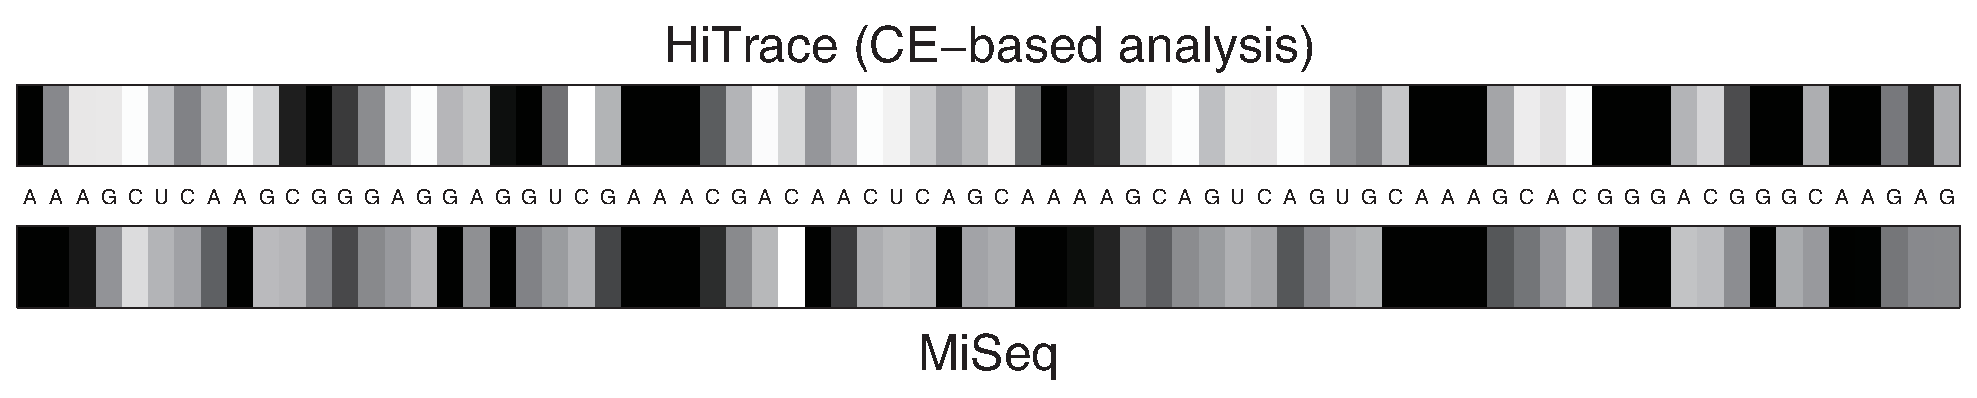
\includegraphics[width=\linewidth]{../figures/reactivities}
\caption{Heatmaps those represent the reactivity values obtained by CE-based analysis and MiSeq, respectively. The data set used is 'C-BACK' sequence.}
\label{f:reactivity-comparison}
\end{figure}
%%%%%%%%%%%%%%%%%%%%%%%%%%%%%%%%%%%%%%%%%%%%%%%%%%%%%%%%%%%%%%%%%%%%%%%%%%%%%%%

\subsection{Reactivity comparison with miseq}
For the final step of verification, we compared the reactivity data obtained by using the proposed method in conjunction with HiTrace, with that obtained by using MiSeq method. In spite of their separated experimental samples and environments, the two reactivity data sets share a same trend as shown in Figure~\ref{f:reactivity-comparison}, evidencing the consistency between the two distinct analyses in terms of their final results.

\end{comment}
